%==============================================================================
\chapter{Model validation: encoding $\Ca$ transient variations to map drugs 
effects on whole-cell to whole-organ in the healthy rat 
heart}\label{cha:chapter6}
%==============================================================================


% %
% %
% \section{Encoding calcium transient variations}
% We used a $4$-feature parametric representation of the calcium transient that maps to common experimentally measured features. The calcium transient was characterised using diastolic concentration ($\dca$), amplitude ($\ampl$), time to peak concentration ($\tp$) and time to half-relaxation from peak concentration ($\rtf$) features. We wish to sample random sets of these features such that the final samples will uniformly cover the feature space, in order to possibly cover both healthy and pathological calcium transient phenotypes. For this purpose, we used linear weighs to scale each of the four features from a representative calcium transient. This parametric encoding of calcium transient variation ensured that all transients maintained a characteristic calcium transient morphology.

% \vspace{0.2cm}
% The specific implementation of this scaling strategy is presented in Alg.~\ref{alg:cascaling}. Note that \texttt{features} function returns the set of four features given an input calcium transient; \texttt{concatenate} function returns a $1$D array obtained as the horizontal stack of the given input row $1$D arrays; \texttt{linear\_interpolator} function returns a function whose call method uses $1$D linear interpolation to find the value of new points.

% \begin{algorithm}
%     \caption{Scaling a representative calcium transient (y:=$\Cai(t)$) using linear interpolation.}\label{alg:cascaling}
%     \begin{algorithmic} 
%     \REQUIRE $t=(t_1,\,\dots,\,t_N),\,y=(y_1,\,\dots,\,y_N),\,\,\textrm{with}\quad t_i,\,y_i\ge 0\,\,\forall\,\,i=1,\dots,\,N$ \\ $p=(p_1,\,\dots,\,p_4),\,\,\textrm{with}\quad p_i\ge 0\,\,\forall\,\,i=1,\dots,\,4$
%     \ENSURE $y_{new}\,\,|\,\,(\textrm{features}(t,\,y_{new}))_{i} = p_i\cdot(\textrm{features}(t,\,y))_{i}\quad\forall\,\,i=1,\dots,4$ \\ $\textrm{where}\,\,\textrm{features}(t,\,y) = (\dca,\,\ampl,\,\tp,\,\rtf)$ \\ \vspace{0.2cm}
%     \STATE $\dca\,\,\leftarrow\,\,(\textrm{features}(t,\,y))_1$
%     \STATE $y_{new}\,\,\leftarrow\,\,p_1\cdot\dca + p_2\cdot(y-\dca)$
%     \STATE $i_{max}\,\,\leftarrow\,\,\argmax\limits_{i=1,\dots,\,N}{y}$
%     \STATE $T \leftarrow t_{N}$ \\
%     \vspace{0.2cm}
%     \IF{$\,\, p_3\cdot(t_{i_{max}} - t_{1}) + p_4\cdot(t_{N}-t_{i_{max}})\le T\,\,$}
%     \STATE $s\,\,\leftarrow\,\,(p_3 - p_4)\cdot t_{i_{max}}$
%     \STATE $t_{tmp}\,\,\leftarrow\,\,\textrm{concatenate}(p_3\cdot (t_{1},\,\dots,\,t_{i_{max}}),\,\,(p_4\cdot t_{i_{max}+1}+s,\,\dots,\,p_4\cdot t_{N-1}+s),\,\,(t_{N}))$
%     \STATE $f\,\,\leftarrow\,\,\textrm{linear\_interpolator}(t_{tmp},\, y_{new})$
%     \STATE $y_{new}\,\,\leftarrow\,\,f(t)$
%     \ELSE
%     \PRINT ``Not a valid scaling! Returning original calcium curve."
%     \STATE $y_{new}\,\,\leftarrow\,\,y$
%     \ENDIF
%     \RETURN $y_{new}$
%     \end{algorithmic}
% \end{algorithm}

% \vspace{0.2cm}
% Fig.~\ref{fig:algintopractice} shows how the algorithm works and how new random calcium transients can be generated.

% \begin{figure}[!ht]
%     \caption{A $4$-feature parametric representation of the calcium transient. (A.1) The calcium transient is described by four relevant quantities: diastolic concentration ($\dca$), amplitude ($\ampl$), time to peak concentration ($\tp$) and time to half-relaxation from peak concentration ($\rtf$). (B.1--4) Each of the $4$ calcium features can be scaled independently to produce a new calcium transient. (A.2) All the features can be scaled at the same time to produce many different new calcium transients.}
%     \centering
%     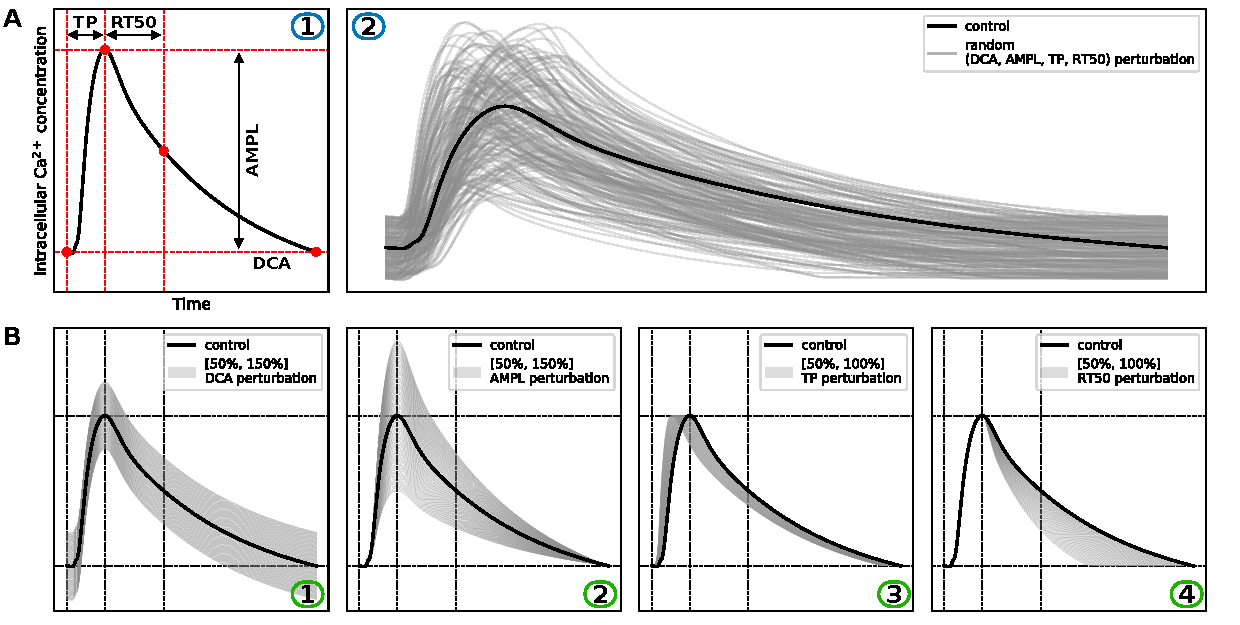
\includegraphics[width=\textwidth]{figures/chapter06/ca_biomarkers_and_scaling_explained_with_labels.pdf}
%     \label{fig:algintopractice}
% \end{figure}

% \vspace{0.2cm}
% An important property of this calcium scaling strategy is that the features scale linearly with the scaling coefficient used, as shown in Fig.~\ref{fig:scalersvscafeatures}. This allows us to randomly sample the scalar parameters that encode the calcium transient from a space filling design (e.g. a Latin hypercube) while generating samples that cover the full feature space. Having a training dataset with input parameters that uniformly cover the high-dimensional parameter space also helps Gaussian process emulators training while at the same time improving their prediction accuracy.

% \begin{figure}[!ht]
%     \centering
%     \caption{{\bf Calcium transient features linearly scale with their respective scaling coefficients.} Example showing $[\SI{50}{\percent},\,\SI{150}{\percent}]$ perturbation for all the calcium features but $\rtf$, which undergoes a $[\SI{50}{\percent},\,\SI{110}{\percent}]$ perturbation.}
%     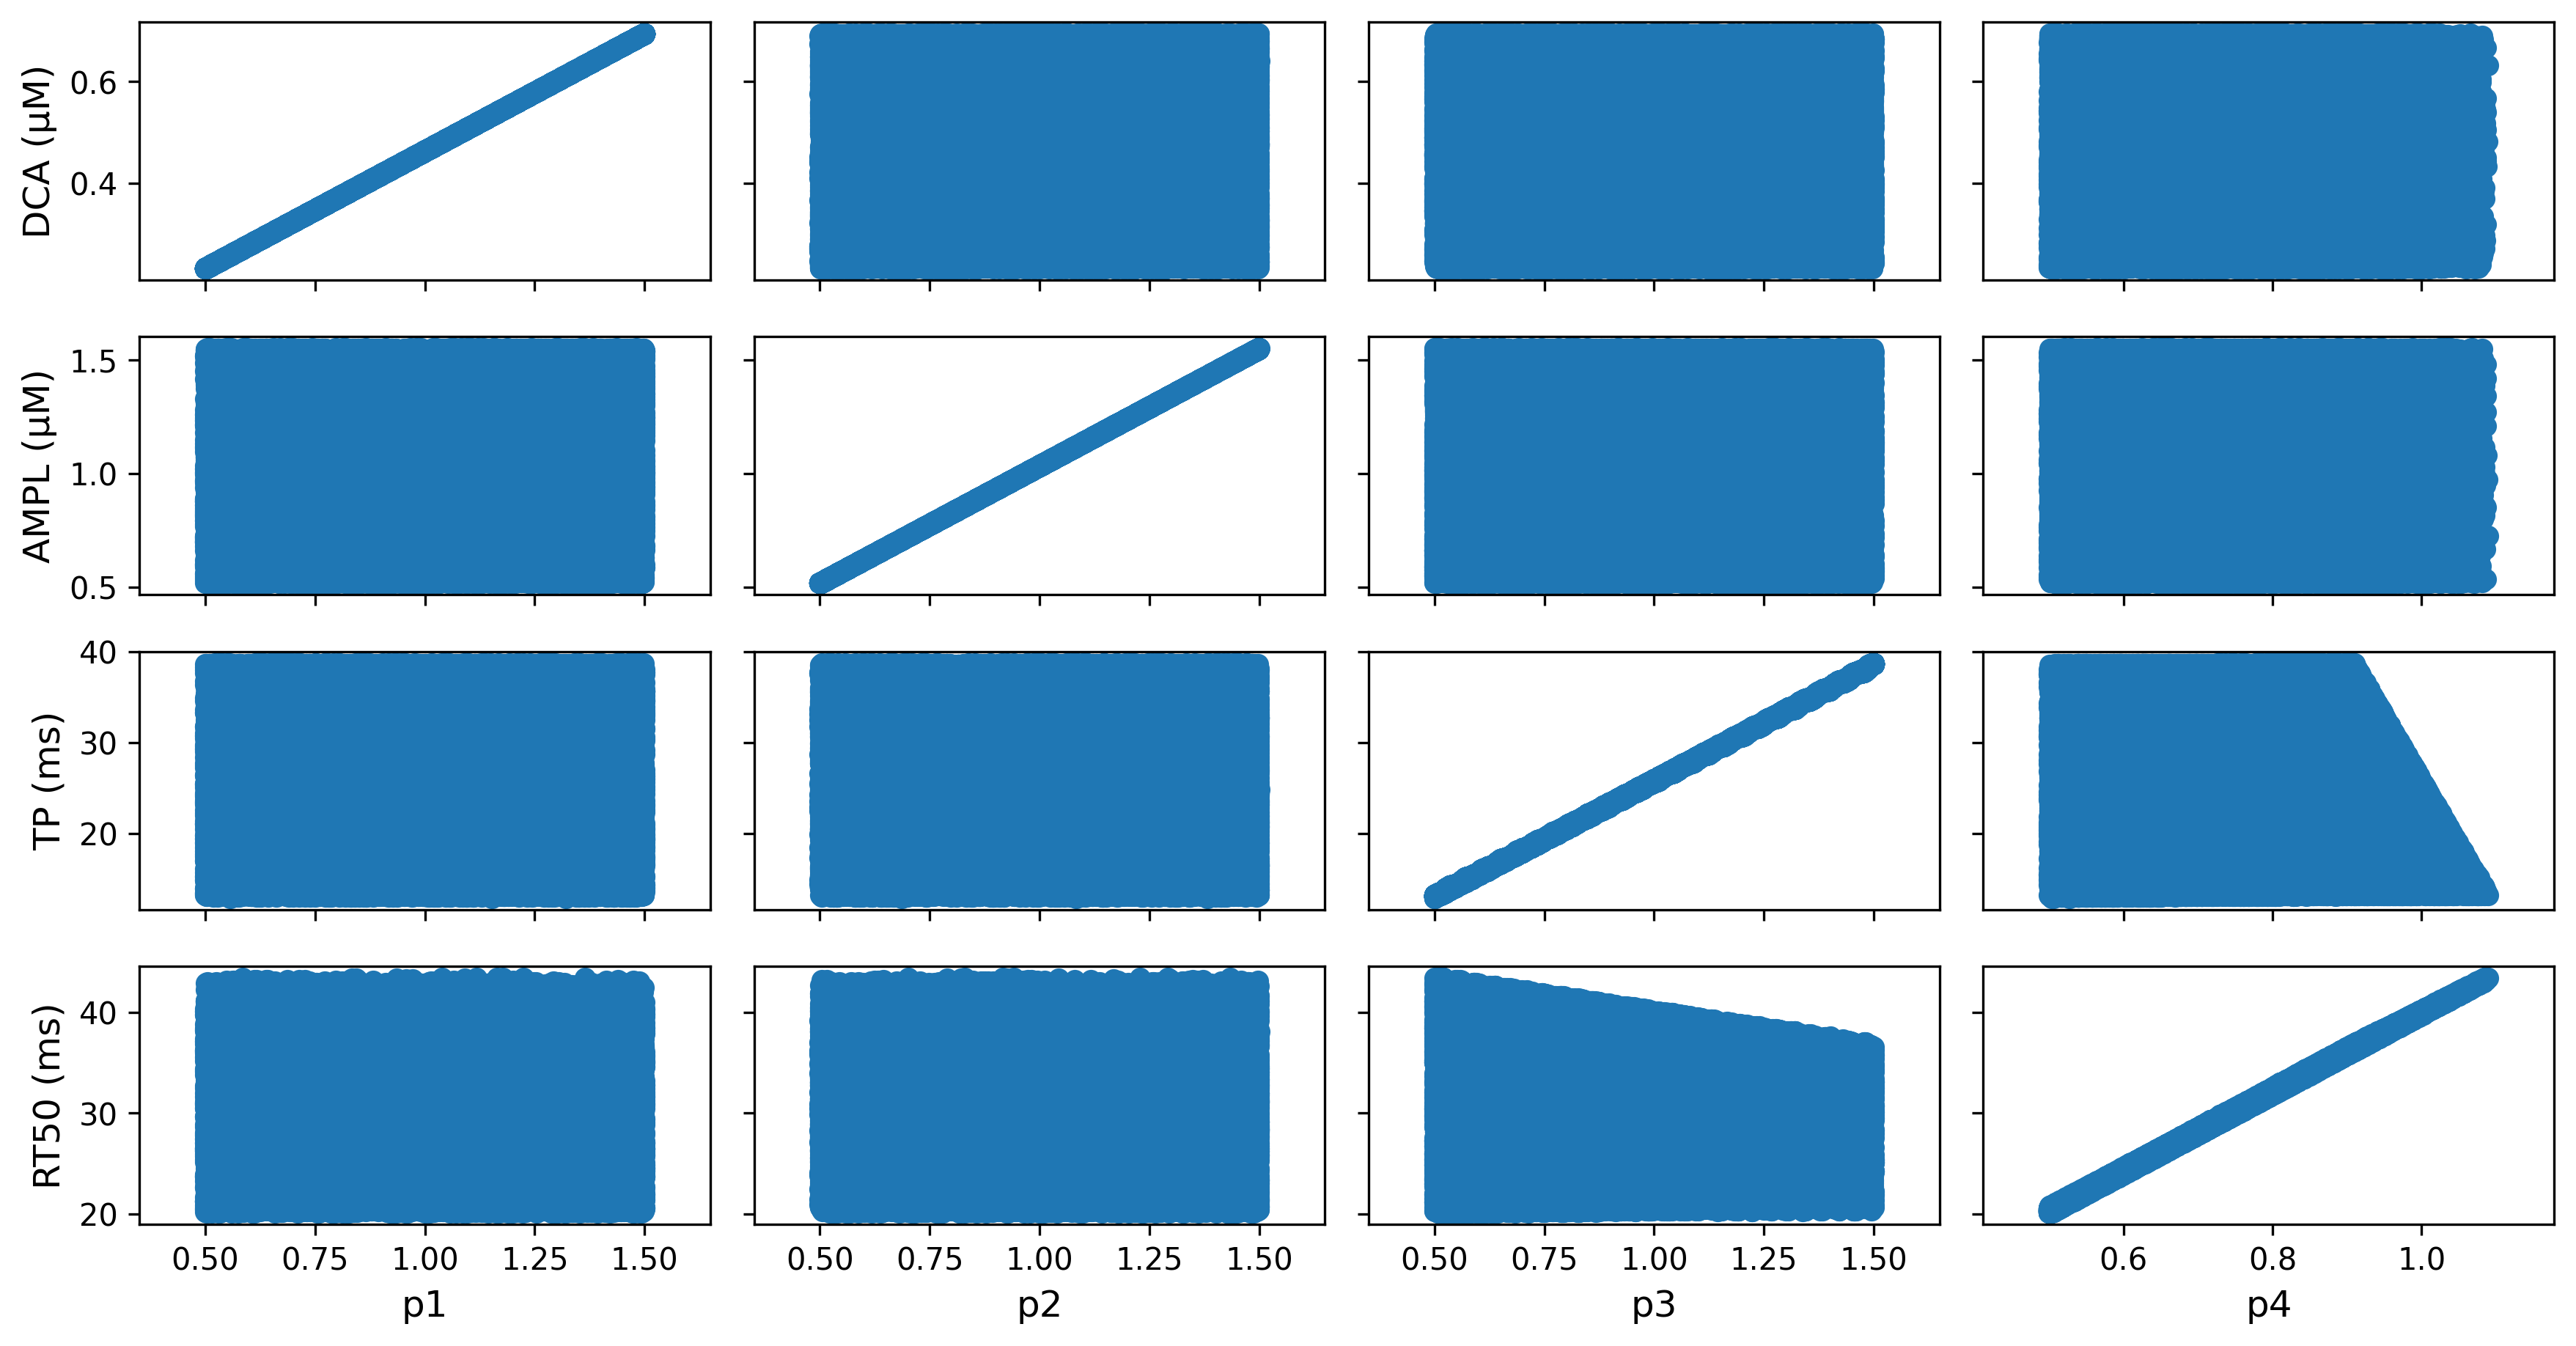
\includegraphics[width=\textwidth]{figures/chapter06/p_vs_b.png}
%     \label{fig:scalersvscafeatures}
% \end{figure}

% \vspace{0.2cm}
% The employed ionic model generates a calcium transient for a fixed pacing rate ($\SI{6}{Hz}$), so that it occurs within a fixed time span. At physiological pacing rates, the rat calcium transient never reaches an equilibrium in diastole, so that during a calcium transient time is spent rising or relaxing. As the cell is paced at a fixed cycle length, the sum of time to peak and relaxation time is capped. This means that one cannot increase without the other decreasing, and independent perturbation of $\tp$ and $\rtf$ can only decrease. If relaxation does interdependently slow, this will mean that the cell will not have enough time to fully relax, and this effect is captured by elevating $\dca$ while decreasing $\ampl$. From an algorithmic view point, not all the randomly picked calcium features' scaling coefficient sets will therefore be viable. The ``if" statement in Alg.~\ref{alg:cascaling} controls this behaviour by discarding all those curves that decay outside the fixed time interval without fully repolarising.

% \vspace{0.2cm}
% The existing coupling between $\tp$ and $\rtf$ calcium features manifests as regions of the feature space that can not be captured by our calcium transient scaling strategy. These are indiecated by the blank triangels in the $p_3$-vs-$\rtf$ and $p_4$-vs-$\tp$ subplots, visible in Fig.~\ref{fig:scalersvscafeatures}.


% \subsection{Model validation}\label{sec:validmethod}
% To test if the rat heart contraction model and its probabilistic surrogate can predict how changes in calcium transients impact the whole heart function, we validated the computational framework by comparing qualitative measurements and predictions of changes in cardiac mechanics in the presence of drugs that manipulate the calcium transient. This provides a multi-scale test on the ability of the model to map from changes in ion channels conductances to changes in calcium transient and the resulting changes in whole heart function. The validation workflow is summarised in Fig.~\ref{fig:validationschematic}.

% \begin{figure}[ht!]
%     \centering
%     \caption{{\bf Model validation workflow.} (1) The pore block model is used to calculate the fraction of blocked ion channel at a given drug concentration for each ion channel. The same channels conductances are scaled to reflect this drug effect and (2) the rat myocyte electrophysiological model is run to generate perturbed calcium transients for different drug concentrations. (3) The calcium transients are used as an input for the $3$D biventricular rat heart contraction model and as many LV features' perturbed values are obtained as the number of input curves, which corresponds to the number of tested drug concentrations. (4) Each LV feature values are plotted against the tested drug concentrations to obtain dose-response curves. (5) The qualitative trend of the LV features after \emph{in silico} drug ``administration'' is compared with literature experimentally measured same drug effects on the same LV features for all the drugs under study.}
%     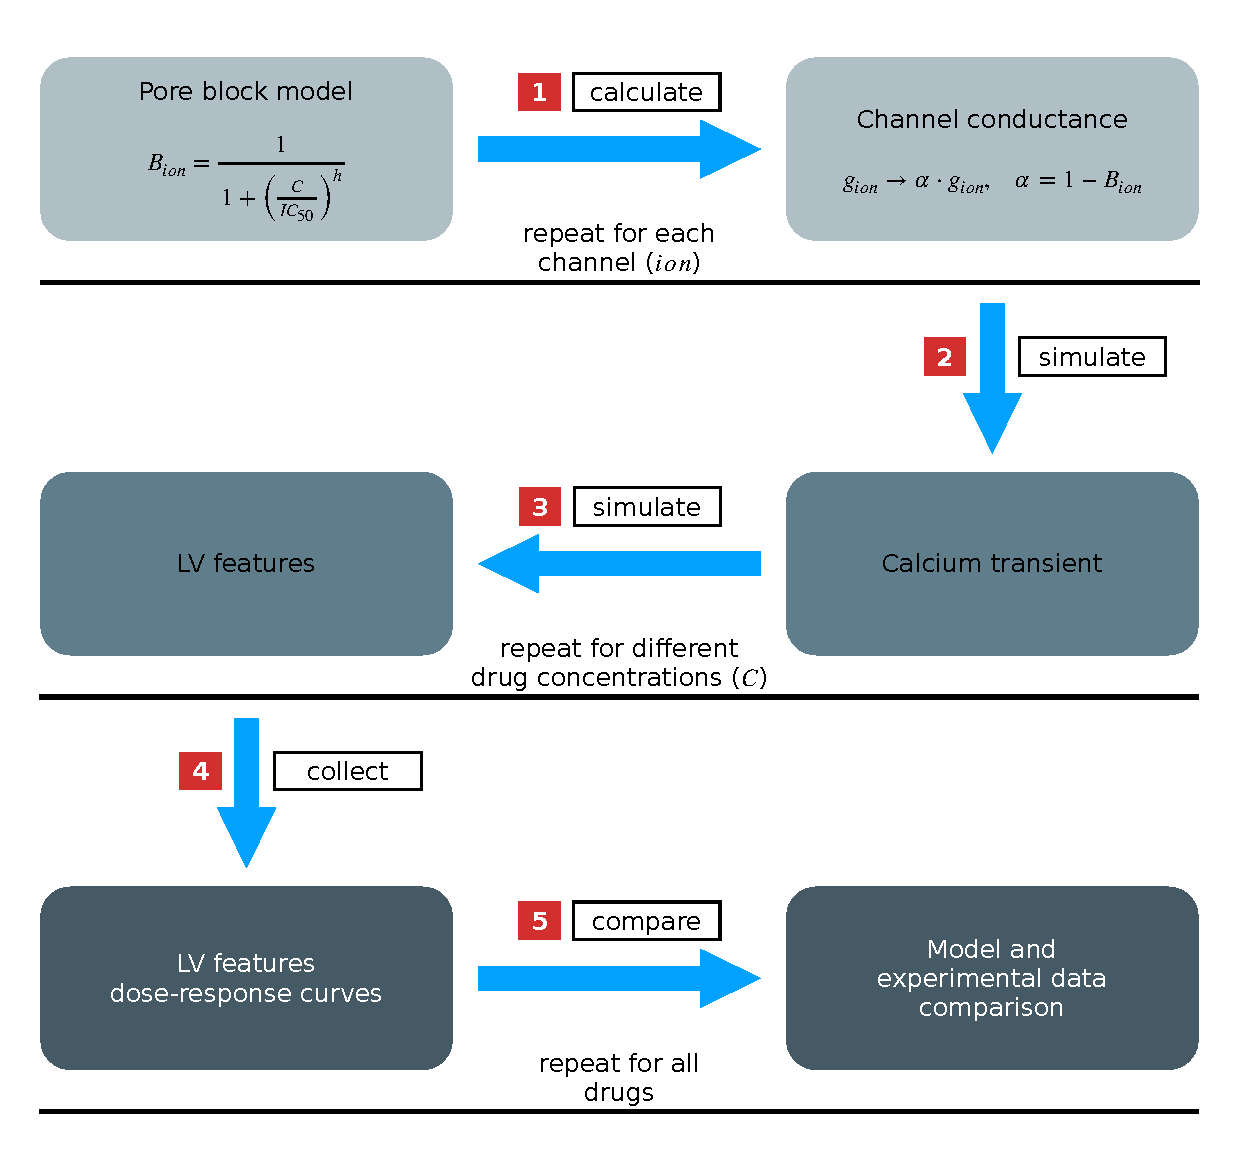
\includegraphics[width=\textwidth]{figures/chapter06/model_validation_schematic.pdf}
%     \label{fig:validationschematic}
% \end{figure}

% \vspace{0.2cm}
% Briefly, we selected $8$ compounds, which were well characterised for multiple ion channels and for which we could find whole organ measurements from literature, from the comprehensive in vitro proarrhythmia assay (CiPA)~\cite{Park:2019} official list, namely bepridil, chlorpromazine, diltiazem, mexiletine, nifedipine, ranolazine, sotalol and verapamil, and we described their action at the cell level using a 4-channel description, namely I\textsubscript{Na}, I\textsubscript{to}, I\textsubscript{K1} and I\textsubscript{CaL}. I\textsubscript{Kr} channel was not included as it has a small amplitude in rats myocytes~\cite{Wymore:1997} and so was not included in the employed rat cell model~\cite{Gattoni:2017}.

% \vspace{0.2cm}
% The affinity of each compound for each channel was taken from CiPA project datasets~\cite{Li:2018, Li:2019} (summarised in~\nameref{S4_Text}) and is described by the Hill coefficient $h$ and the half-maximal inhibitory concentration $\icf$ values of a Hill-type relationship which gives the fraction of blocked current $B$ as a function of the drug concentration $C$, also known as pore block model:
% %
% \begin{equation}
%     B = \frac{1}{1+\left(\frac{C}{\icf}\right)^h}
% \end{equation}

% \noindent
% For each given drug, we calculated $B$ for each channel when $C$ was set to equally-spaced values in a log-molar space. By subtracting the obtained $B$ values from $1$, we obtained a matrix of scaling coefficients for the channels' conductances, representing the fractions of active channels in the presence of the drugs at different concentrations. We tested $13$ equally-spaced drug concentrations ($-\log{\SI{}{\Molar}}$) in the range $[4,\,10]$ (extremes included), which corresponded to drugs concentrations between $\SI{e-10}{\Molar}$ and $\SI{e-4}{\Molar}$. We then run the Gattoni et al.~\cite{Gattoni:2017} model by scaling the ion channels conductances to simulate the action of different concentrations of each drug at the cell level and collected the resulting calcium transients (last beat curves of stead-state, $5000$ beats simulations). An example of calcium transients obtained after simulating the effect of verapamil is provided in~\nameref{S4_Text}. The used approach simulates the drug induced changes in calcium transients, thereby overcoming the issue when no directly recorded calcium transients are available. In so doing, we created a fully simulated map from drug properties to whole organ function.


% \vspace{0.2cm}
% We used the full multi-scale model (Section~\ref{sec:ratmodel}) to simulate the LV features values using as an input the obtained calcium transients and the remaining parameters fixed to the SHAM rat model reference values. This allowed us to obtain the LV features' change from baseline values in a dose-dependent manner. PeakP, maxdP and mindP features' simulated responses to different doses of all the tested drugs are reported in~\nameref{S4_Text}. These features' qualitative responses after \emph{in silico} drug ``administration'' were compared to qualitative changes in the same LV features observed after drugs administration in literature experimental studies performed on either conscious, or Langendorff-perfused or working healthy rat heart preparations. These experimental changes were either recorded after a single dose in the pre-ischemic phase of an ischemia-reperfusion experiment, or in a dose-dependent manner, and are summarised in~\nameref{S4_Text}.


% %
% %
% %
% % \section{Incorporating the Calcium transient}
% % We used a $4$-features (discrete) representation of the calcium transient to be included in our emulating framework. In particular, we characterised the calcium transient using diastolic concentration (DCA), amplitude (AMPL), time to peak concentration (TP) and time to half-relaxation from peak concentration ($\textrm{RT}_{50}$) features. We used simple linear interpolation to scale these four characteristics linearly with the scaling coefficient used (Figure~\ref{fig:scalersvscafeatures}). This ensured that when sampling sets of scalers from a space-filling design, the respectively obtained calcium transient curves had features which were again uniformly distributed on and covering the entire calcium features space. As we saw previously in the case of mechanics parameters only, this is a required property for sampled (finite) space to be a good representation of the entire parameter space to be then used for training. It is worth mentioning that ensuring this property is non-trivial: commonly used phenomenological calcium formulations such as the bi-exponential curve rise-decay phases representation~\cite{Rice:2008} cannot achieve a scaler-feature linear relationship although being regulated by the same number of parameters corresponding to characterisations of the same calcium transient's features. The algorithm is presented in Algorithm~\ref{alg:cascaling}.

% % Because of a physical constraint on the time interval the calcium transient curve is bound to when the cell is paced at $\SI{6}{Hz}$ (which is the physiological pacing rate for a healthy rat heart) not all the calcium features' scaling coefficient sets will be viable. The ``if" statement in Algorithm~\ref{alg:cascaling} in fact discards all those curves that decay outside the fixed time interval without fully repolarising. This is our modelling design choice as we believe that at steady-state, these non-repolarising curves will still be captured by our calcium features description, corresponding to a higher DCA and a lower RT50 features values. We can now explain the triangularly-shaped parameter regions cut off the $p_3$-vs-$\rtf$ and $p_4$-vs-$\tp$ subplots seen in Figure~\ref{fig:scalersvscafeatures}: when increasing the time to peak calcium concentration the calcium transient has less time to fully repolarise, so this kind of perturbation is only viable if we at the same time lower the time to half-maximal relaxation; conversely when increasing the time to half-maximal relaxation the calcium transient needs to start decaying earlier, so this kind of perturbation is only viable if we at the same time lower the time to peak calcium concentration.


% %
% %
% %
% \section{CiPA compounds}
% To test if the virtual rat heart can predict how changes in calcium transients impact whole heart function, we validated the model by comparing qualitative measurements and predictions of changes in cardiac mechanics in the presence of drugs that manipulate the calcium transient. This provides a multi-scale test on the ability of the model to map from changes in ion channels conductances to changes in calcium transient and the resulting changes in whole heart function.

% We selected $8$ compounds (which were well characterised for multiple ion channels and for which we could find whole organ measurements from literature) from the comprehensive in vitro proarrhythmia assay (CiPA)~\cite{Park:2019} official list, namely bepridil, chlorpromazine, diltiazem, mexiletine, nifedipine, ranolazine, sotalol, verapamil, and we described their action at the cell level using a 4-channel (I\textsubscript{Na}, I\textsubscript{to}, I\textsubscript{K1} and I\textsubscript{CaL}) description. I\textsubscript{Kr} channel was not included due to its absence in the employed rat cell model~\cite{Gattoni:2017}. The affinity of each compound for each channel was also taken from the official CiPA program datasets (\nolinkurl{https://github.com/FDA/CiPA/blob/Model-Validation-2018/AP_simulation/data/newCiPA.csv}~\cite{Li:2019}) and given by the Hill coefficient $h$ and the half-maximal inhibitory concentration $IC_{50}$ values of a Hill-type relationship which describes the fraction of blocked current $B$ as a function of the drug concentration $C$, also known as pore block model:
% %
% \begin{equation}
%     B = \frac{1}{1+\left(\frac{C}{IC_{50}}\right)^h}
% \end{equation}

% \noindent
% The Hill coefficient and $IC_{50}$ values for the selected drug are summarised in Table~\ref{tab:drugporeblock}. An example of the blocking affinity between verapamil and the ion channels is shown in Figure~\ref{fig:poreblockverapamil}.

% \begin{table}[hbt!]
%     \myfloatalign
%     \begin{tabularx}{\textwidth}{lllll}
%     \toprule
%     \tableheadline{Drug} & \multicolumn{4}{c}{\spacedlowsmallcaps{Ion channel}} \\
%     \midrule
%     & \tableheadline{I\textsubscript{Na}} & \tableheadline{I\textsubscript{to}} & \tableheadline{I\textsubscript{K1}} & \tableheadline{I\textsubscript{CaL}} \\
%     \midrule
%     \tableheadline{bepridil}  & & & & \\
%     $IC_{50}$ ($\SI{}{\nano\Molar}$)     & $2.93\cdot10^{3}$ & $8.59\cdot10^{3}$ & $0$ & $2.81\cdot10^{3}$ \\
%     h                               & $1.16$ & $3.54$ & $0$ & $0.65$ \\ \midrule
%     \tableheadline{chlorpromazine}  & & & & \\
%     $IC_{50}$ ($\SI{}{\nano\Molar}$)     & $4.54\cdot10^{3}$ & $1.76\cdot10^{7}$ & $9.27\cdot10^{3}$ & $8.19\cdot10^{3}$ \\
%     h                               & $2.00$ & $0.37$ & $0.69$ & $0.84$ \\ \midrule
%     \tableheadline{diltiazem}       & & & & \\
%     $IC_{50}$ ($\SI{}{\nano\Molar}$)     & $1.11\cdot10^{5}$ & $2.82\cdot10^{9}$ & $0$ & $1.12\cdot10^{2}$ \\
%     h                               & $0.70$ & $0.17$ & $0$ & $0.71$ \\ \midrule
%     \tableheadline{mexiletine}      & & & & \\
%     $IC_{50}$ ($\SI{}{\nano\Molar}$)     & $0$ & $0$ & $0$ & $3.82\cdot10^{4}$ \\
%     h                               & $0$ & $0$ & $0$ & $1.03$ \\ \midrule
%     \tableheadline{nifedipine}      & & & & \\
%     $IC_{50}$ ($\SI{}{\nano\Molar}$)     & $2.84\cdot10^{4}$ & $0$ & $0$ & $1.15\cdot10^{1}$ \\
%     h                               & $1.11$ & $0$ & $0$ & $0.67$ \\ \midrule
%     \tableheadline{ranolazine}      & & & & \\
%     $IC_{50}$ ($\SI{}{\nano\Molar}$)     & $6.88\cdot10^{4}$ & $0$ & $0$ & $0$ \\
%     h                               & $1.42$ & $0$ & $0$ & $0$ \\ \midrule
%     \tableheadline{sotalol}         & & & & \\
%     $IC_{50}$ ($\SI{}{\nano\Molar}$)     & $1.14\cdot10^{9}$ & $\SI{4.31e7}{}$ & $3.05\cdot10^{6}$ & $7.06\cdot10^{6}$ \\
%     h                               & $0.51$ & $0.66$ & $1.20$ & $0.87$ \\ \midrule
%     \tableheadline{verapamil}       & & & & \\
%     $IC_{50}$ ($\SI{}{\nano\Molar}$)     & $0$ & $1.34\cdot10^{4}$ & $3.49\cdot10^{8}$ & $2.02\cdot10^{2}$ \\
%     h                               & $0$ & $0.82$ & $0.27$ & $1.10$ \\
%     \bottomrule                          
%     \end{tabularx}
%     \caption{$IC_{50}$ and Hill coefficient values describing the affinity of eight CiPA compounds with the I\textsubscript{Na}, I\textsubscript{to}, I\textsubscript{K1} and I\textsubscript{CaL} ion channels. The null value indicates that the specific compound has no inhibitory effect on the respective ion channel. Values taken from \nolinkurl{https://github.com/FDA/CiPA/blob/Model-Validation-2018/AP_simulation/data/newCiPA.csv}~\cite{Li:2019}.}
%     \label{tab:drugporeblock}
% \end{table}

% % \begin{figure}[hbt!]
% %     \myfloatalign
% %     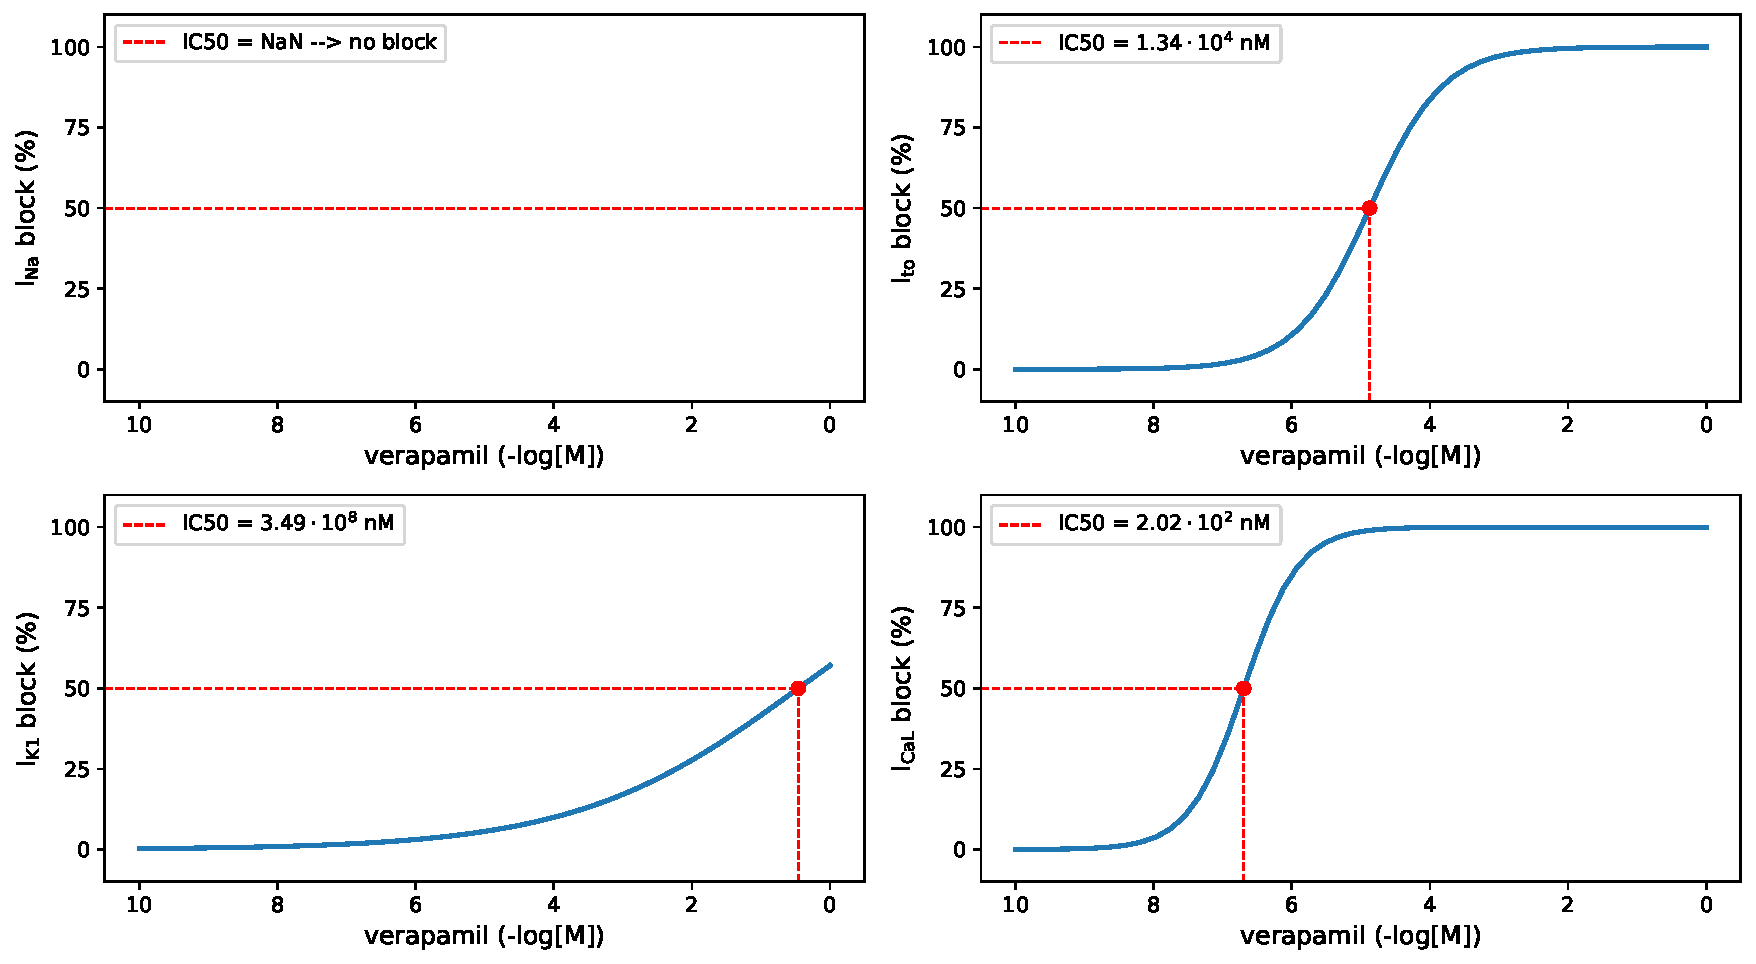
\includegraphics[width=1\textwidth]{figures/chapter06/channels_block_verapamil_drug_conc_response_curve.pdf}
% %     \caption{The pore block model. Example of calculated blocked ion channels' fractions with different concentrations of verapamil.}
% %     \label{fig:poreblockverapamil}
% % \end{figure}

% For each given drug, we calculated the block percentages for each channel when the drug concentration was taking equally-spaced values in a log-molar space. By subtracting these values from $1$, we could finally obtain a matrix of coefficients (Table~\ref{tab:gscalers}) to be used as scalers for each of the channels' conductances, representing the fraction of active channel in the presence of the drugs at different concentrations. We tested $13$ equally-spaced drug concentrations ($-\log{\SI{}{\Molar}}$) in the range $[4,\,10]$ (extremes included), which corresponded to drugs concentrations between $\SI{e-10}{\Molar}$ and $\SI{e-4}{\Molar}$. We then run the Gattoni et al.~\cite{Gattoni:2016} model by scaling the ion channels conductances to simulate the action of different concentrations of each drugs at the cell level and collected the resulting calcium transient (the last beat curve of a stead-state, $5000$ beats simulation). These are displayed in Figure~\ref{fig:calciumverapamil} for verapamil.

% \begin{table}[hbt!]
%     \myfloatalign
%     \begin{tabularx}{\textwidth}{lXXXX}
%     \toprule
%     \tableheadline{Concentration ($\SI{}{\Molar}$)} & \multicolumn{4}{c}{\spacedlowsmallcaps{Channel conductance scaler}} \\
%     \midrule   
%     & \tableheadline{$\alpha_{Na}$} & \tableheadline{$\alpha_{to}$} & \tableheadline{$\alpha_{K1}$} & \tableheadline{$\alpha_{CaL}$} \\
%     \cmidrule{2-5}
%     $\SI{1.00e-10}{}$ & $1.000000$ & $0.999938$ & $0.997356$ & $0.999763$ \\
%     $\SI{3.16e-10}{}$ & $1.000000$ & $0.999840$ & $0.996395$ & $0.999162$ \\
%     $\SI{1.00e-09}{}$ & $1.000000$ & $0.999588$ & $0.995087$ & $0.997044$ \\
%     $\SI{3.16e-09}{}$ & $1.000000$ & $0.998942$ & $0.993308$ & $0.989628$ \\
%     $\SI{1.00e-08}{}$ & $1.000000$ & $0.997285$ & $0.990891$ & $0.964274$ \\
%     $\SI{3.16e-08}{}$ & $1.000000$ & $0.993050$ & $0.987611$ & $0.884191$ \\
%     $\SI{1.00e-07}{}$ & $1.000000$ & $0.982329$ & $0.983170$ & $0.683518$ \\
%     $\SI{3.16e-07}{}$ & $1.000000$ & $0.955806$ & $0.977174$ & $0.379243$ \\
%     $\SI{1.00e-06}{}$ & $1.000000$ & $0.893775$ & $0.969109$ & $0.147353$ \\
%     $\SI{3.16e-06}{}$ & $1.000000$ & $0.765996$ & $0.958315$ & $0.046608$ \\
%     $\SI{1.00e-05}{}$ & $1.000000$ & $0.560152$ & $0.943970$ & $0.013640$ \\
%     $\SI{3.16e-05}{}$ & $1.000000$ & $0.331306$ & $0.925072$ & $0.003897$ \\
%     $\SI{1.00e-04}{}$ & $1.000000$ & $0.161604$ & $0.900474$ & $0.001105$ \\
%     \bottomrule
%     \end{tabularx}
%     \caption{Active fractions of the I\textsubscript{Na}, I\textsubscript{to}, I\textsubscript{K1} and I\textsubscript{CaL} ion channels calculated using the pore block model for different drugs (verapamil as an example) concentrations. For each ion channel the scaler $\alpha_{ion}$ is multiplied to the respective conductance ($\alpha_{ion}\cdot g_{ion}$) to simulate the inhibitory effect of the drug.}
%     \label{tab:gscalers}
% \end{table}

% % \begin{figure}[hbt!]
% %     \myfloatalign
% %     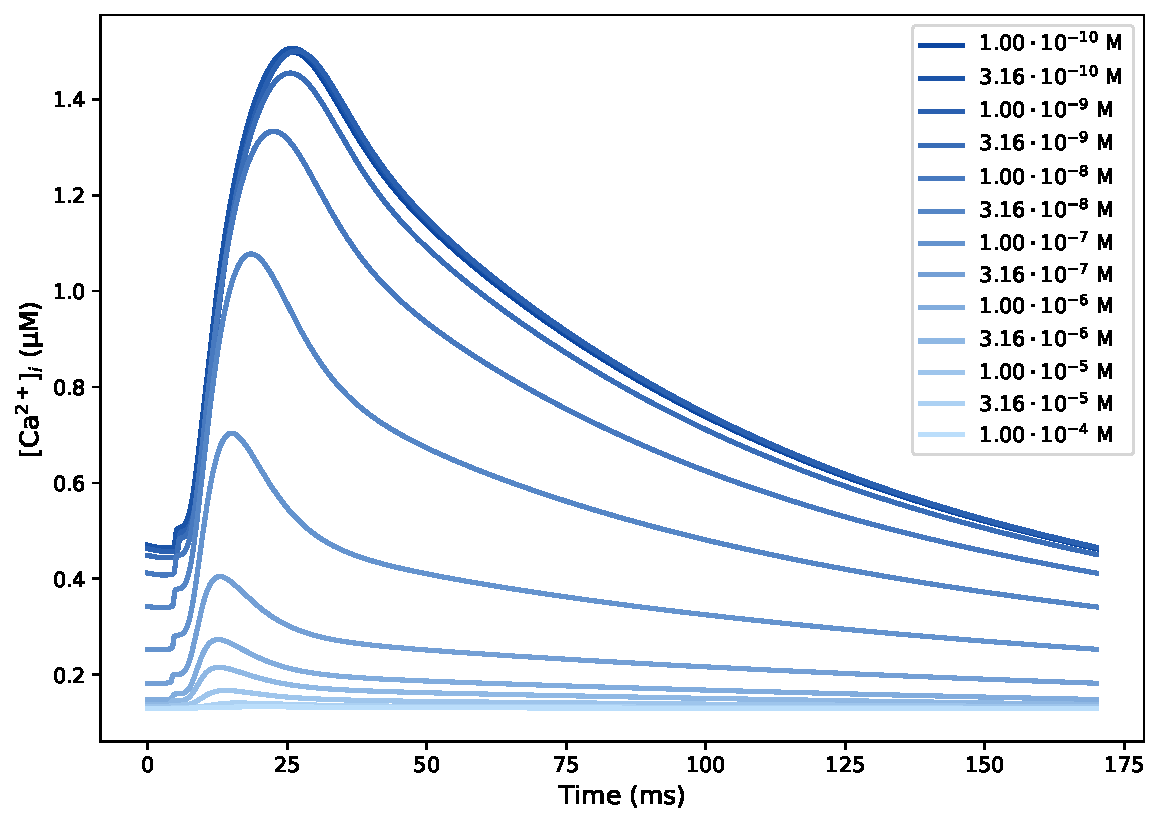
\includegraphics[width=1\textwidth]{figures/chapter06/verapamil_calcium_curve_drug.pdf}
% %     \caption{The effect of verapamil on intracellular calcium transient. Gattoni et al.~\cite{Gattoni:2016} model is run using different ion channels conductances' scalers (each row of Table~\ref{tab:gscalers}) to simulate the effect of different concentrations (blue colour variants) of the example drug considered.}
% %     \label{fig:calciumverapamil}
% % \end{figure}

% The calcium transients obtained in the presence of the drug at different concentrations were encoded by the presented $4$ features of interest: $\dca$, $\ampl$, $\tp$ and $\rtf$. This means we can plot dose-response curves of the calcium transient features (Figure~\ref{fig:cafeatsverapamilrespcurve}).

% % \begin{figure}[hbt!]
% %     \myfloatalign
% %     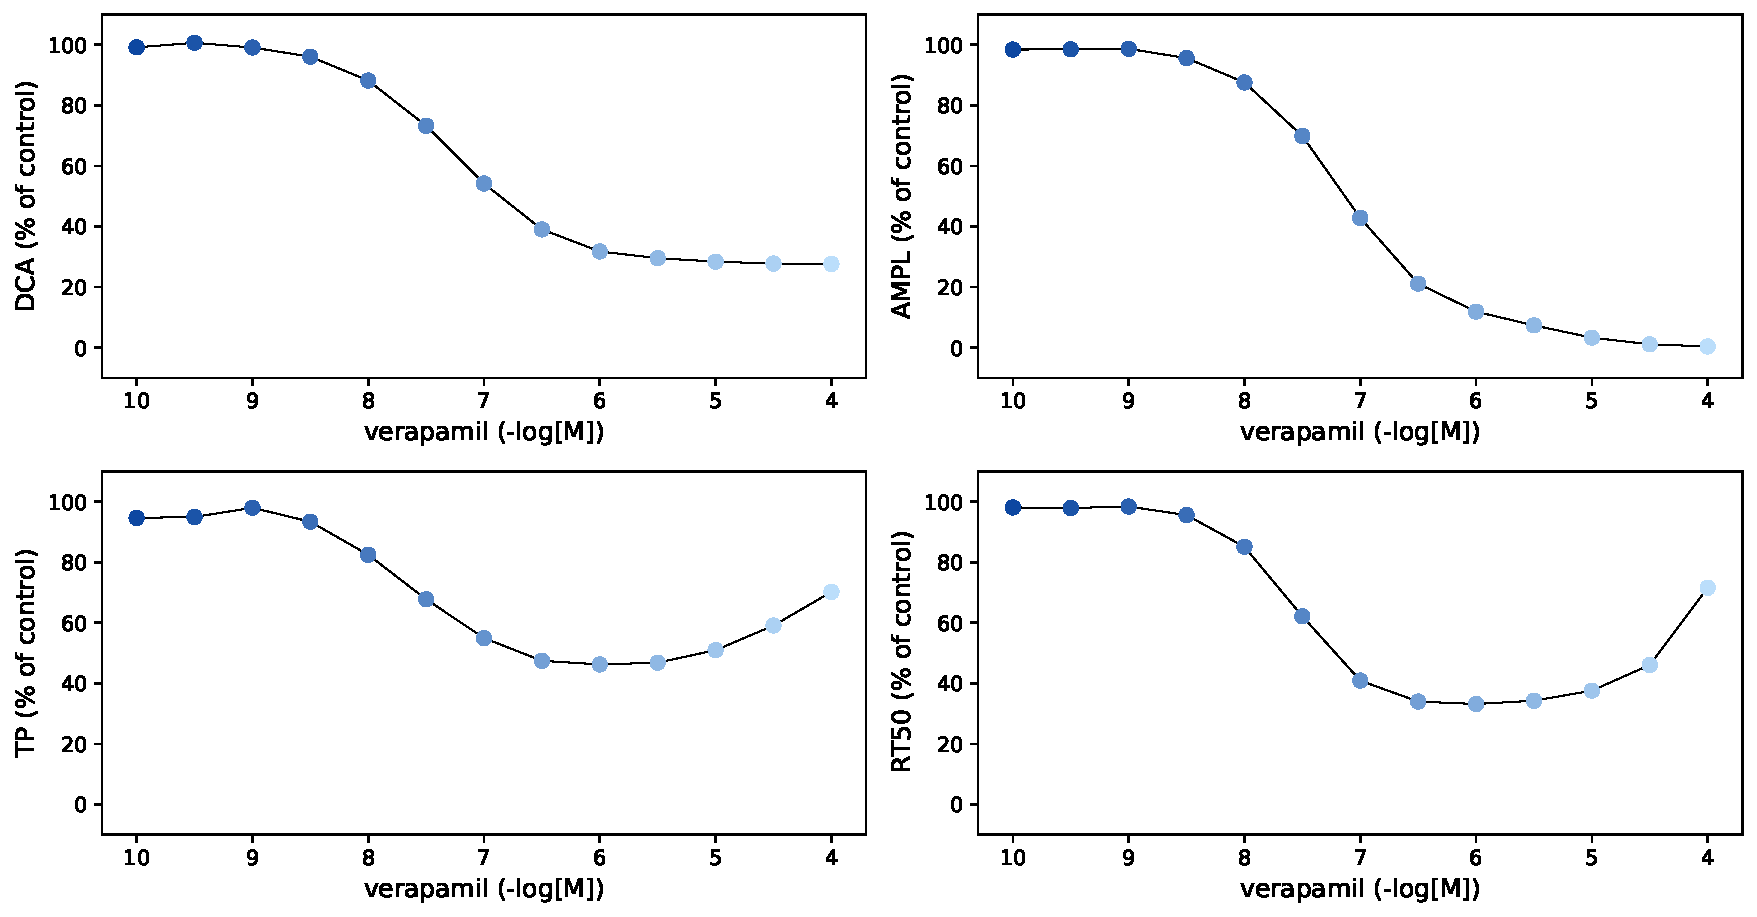
\includegraphics[width=1\textwidth]{figures/chapter06/verapamil_dose_calcium_response_curve_drug.pdf}
% %     \caption{Calcium transient features dose-response curves.}
% %     \label{fig:cafeatsverapamilrespcurve}
% % \end{figure}

% We can notice that in the $\tp$ and $\rtf$ cases the response is not following a fully logistic trend on the right branches. This is because for high drug concentrations we have seen that the calcium signal had almost vanished, making analysis of these curves challenging. However, we can fit a Hill curve (Figure~\ref{fig:cafeatsverapamilrespcurvehillfit}) to the point-wise calculated response-curve after slightly correcting those non-physiological values at the extremes to obtain the percentage from control at whichever dose we wish to query our model.

% % \begin{figure}[hbt!]
% %     \myfloatalign
% %     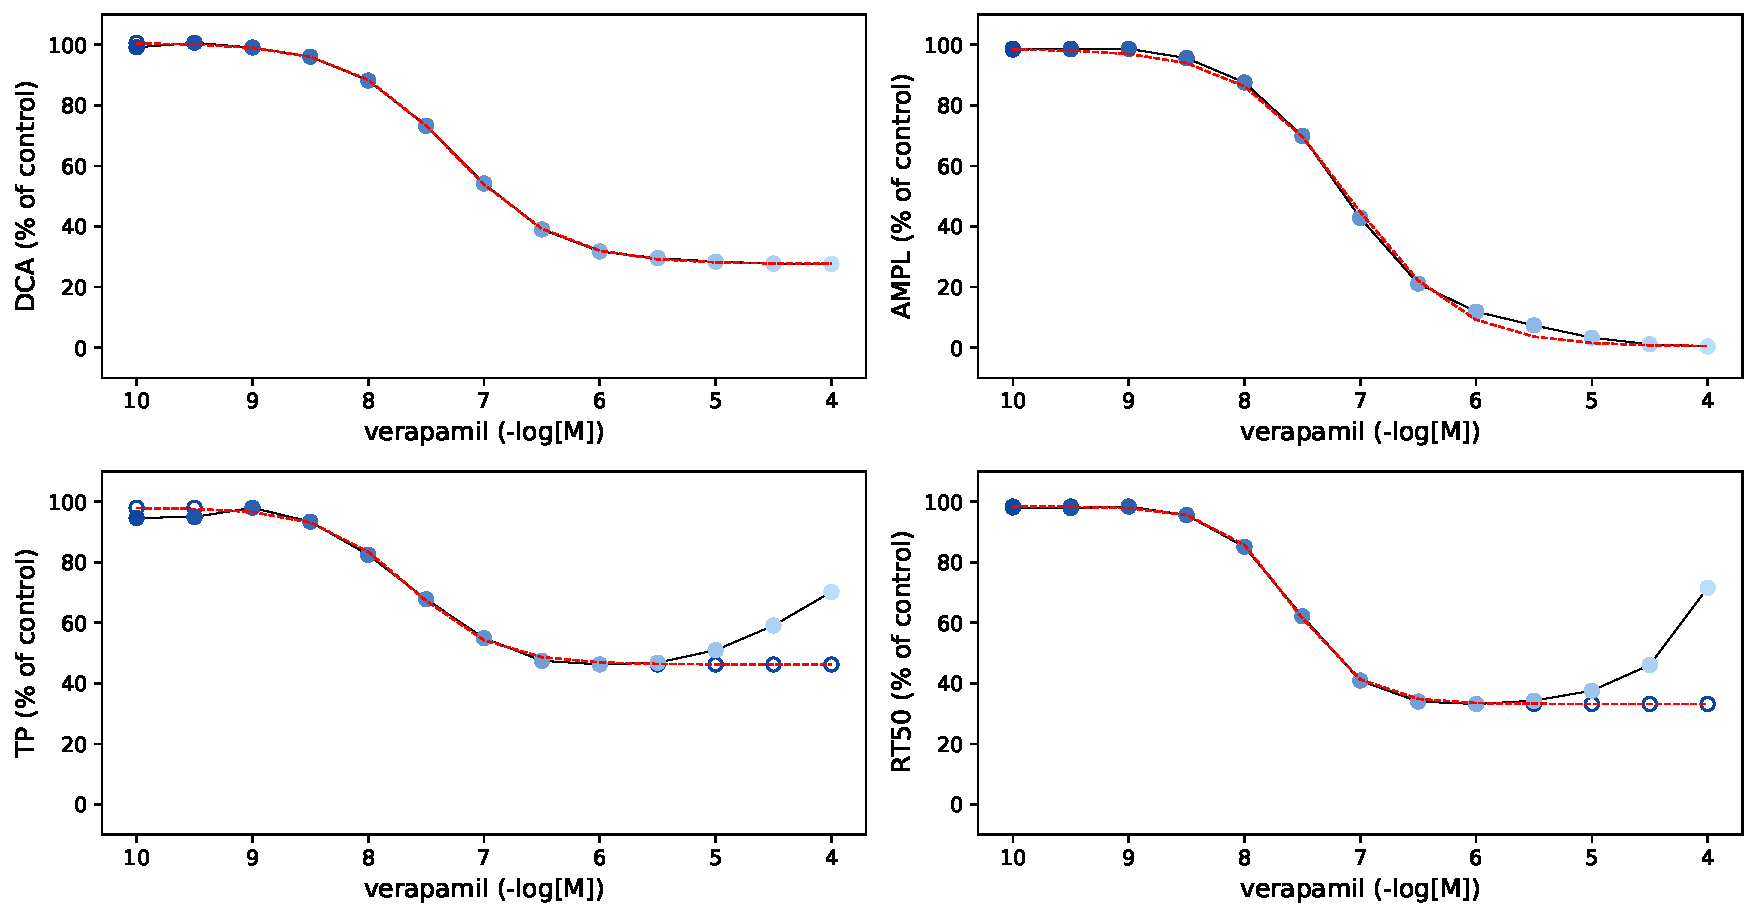
\includegraphics[width=1\textwidth]{figures/chapter06/verapamil_dose_calcium_response_curve_drug_Hill_fit.pdf}
% %     \caption{Hill curve fit to the calcium transient features dose-response curves.}
% %     \label{fig:cafeatsverapamilrespcurvehillfit}
% % \end{figure}

% We aim to validate our emulation framework by showing that we can predict the same qualitative change in the LV features after drug administration observed in the literature. For this purpose, we firstly collected information about known effects of the eight compounds from literature studies performed on Langendorff-perfused healthy rat hearts. We retrieved information for the change in PeakP, maxdP and mindP features either after a single-shot (one dosage) in the pre-ischemic phase of an ischemia-reperfusion experiment, or in a dose-dependent manner. These are summarised in Table~\ref{tab:drugvalidationrefs}.

% \begin{table}[hbt!]
%     \myfloatalign
%     \begin{tabularx}{\textwidth}{lllll}
%     \toprule
%     \tableheadline{Drug}           & \multicolumn{3}{c}{\spacedlowsmallcaps{LV features}} & \tableheadline{References} \\
%     \midrule
%     & PeakP & maxdP & mindP & \\
%     \cmidrule{2-4}
%     \tableheadline{bepridil}       & $\downarrow$ & $\,$ & $\,$ & \cite{Leiris:1984, Amsterdam:1988, Huizer:1987} \\
%     \tableheadline{chlorpromazine} & $\downarrow$ & $\,$ & $\,$ & \cite{Katsuoka:1989, Langslet:1971, Sakai:2017} \\
%     \tableheadline{diltiazem}      & $\downarrow$ & $\downarrow$ & $\downarrow$ & \cite{Flaim:1982, Koltai:1989, Dong:1997} \\
%     \tableheadline{mexiletine}     & $-$ & $-$ & $\,$ & \cite{Kamiyama:1995, Hesketh:2020, Marshall:1981} \\
%     \tableheadline{nifedipine}     & $\downarrow$ & $\downarrow$ & $\downarrow$ & \cite{Dong:1997, Saponara:2007, Nishimura:1992} \\
%     \tableheadline{ranolazine}     & $-$ & $-$ & $-$ & \cite{Wang:2007, Hwang:2009, Wang:2019} \\
%     \tableheadline{sotalol}        & $\downarrow$ & $\downarrow$ & $-$ & \cite{Mackin:2019, Peralta:2000, Hoffmeister:1988} \\
%     \tableheadline{verapamil}      & $\downarrow$ & $\downarrow$ & $\downarrow$ & \cite{Simonovic:2019, Stojic:2017, Kolař:1990} \\
%     \bottomrule
%     \end{tabularx}
%     \caption{Dose-dependent or single-dose change in PeakP, maxdP and mindP LV features observed in literature for eight different CiPA compounds. Down-facing arrow means that the specific LV feature decreases from control values with the specific drug, while dash means that the drug has no effect on that feature. Empty space means that the specific information could not be retrieved from literature.}
%     \label{tab:drugvalidationrefs}
% \end{table}

% We then predicted the LV features at input parameter points which had all the calcium-related parameters scaled to represent the corresponding drug dosage reproduced and the remaining parameters fixed to reference values. The LV features dose-dependent response for verapamil is shown in Figure~\ref{fig:LVfeatsverapamilrespcurve}. A clear trend can be observed for most of the features (e.g. peak systolic pressure decreases with increasing the drug dosage). The GPEs' uncertainties as expected are higher when extrapolating (red shaded areas on the right of the dashed red line) compared to when interpolating (grey shaded areas).

% % \begin{figure}[hbt!]
% %     \myfloatalign
% %     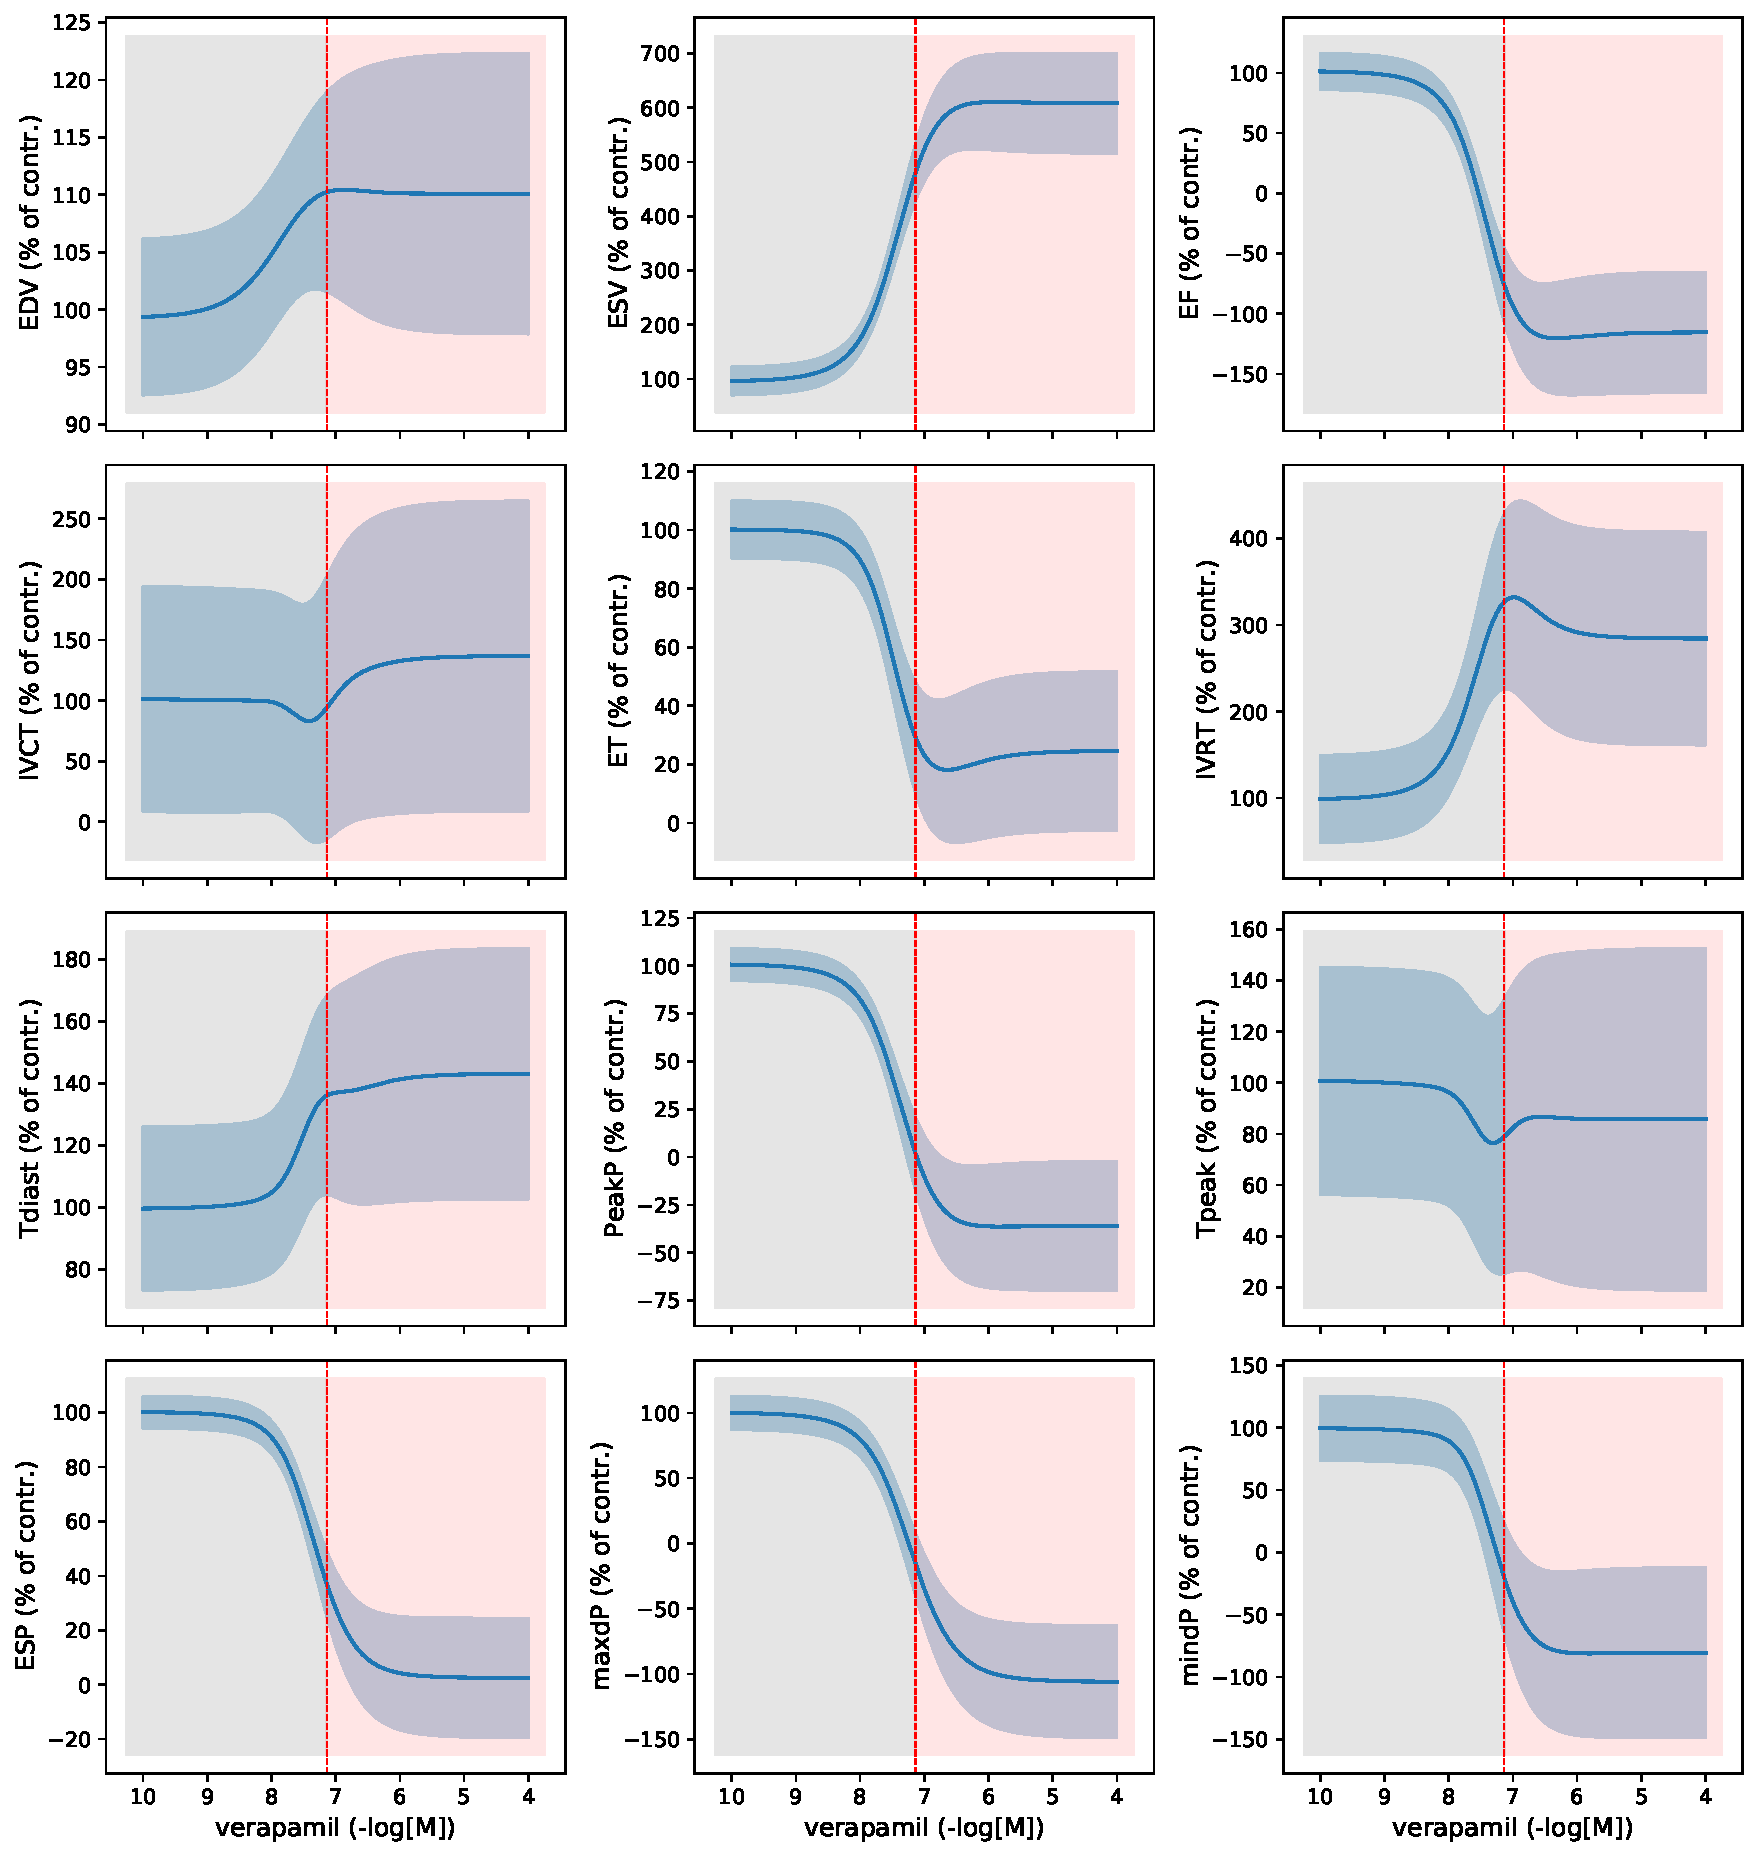
\includegraphics[width=1\textwidth]{figures/chapter06/verapamil_dose_LVfeatures_response_curve_drug.pdf}
% %     \caption{LV features dose-response curves for verapamil. Predicted LV features are displayed (blue line) as percentage of control values. Uncertainties ($2$ std) around the predicted values are given as shaded blue areas. Shaded gray and red (after the dashed red line) areas correspond to regions where the emulators are interpolating and extrapolating, respectively.}
% %     \label{fig:LVfeatsverapamilrespcurve}
% % \end{figure}

% We finally compared the observed LV features' trends with what reported in literature (Table~\ref{tab:drugvalidationrefs}), and this is summarised in~Figure~\ref{fig:validationtable}). The model correctly predicted $15$ out of $19$ experimental observations, matching $6$ out of $8$ compounds. In all cases where the model and data did not match either the data or model predicted no change.

% % \begin{figure}[hbt!]
% %     \myfloatalign
% %     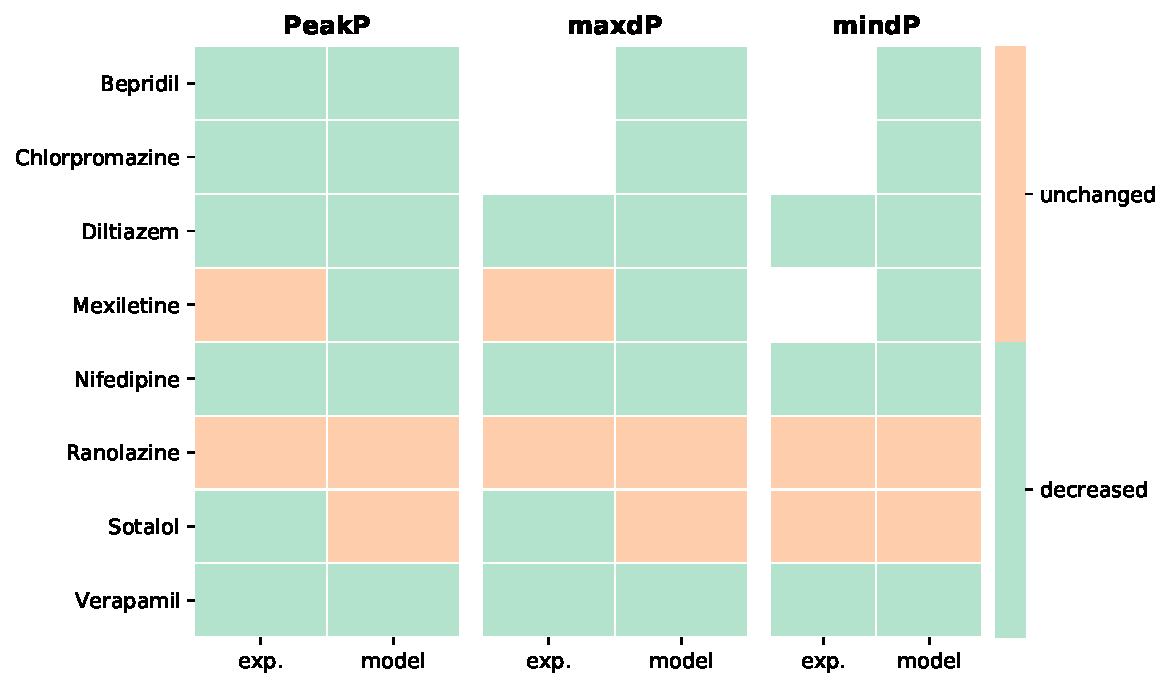
\includegraphics[width=1\textwidth]{figures/chapter06/validation_table.pdf}
% %     \caption{Model validation against known CiPA compounds effects on whole-organ function. Eight CiPA compounds effects ("exp." columns) on peak LV systolic pressure (PeakP) and maximum rates of LV pressure rise, decay (maxdP, mindP) are compared with model same drugs' predicted effects on the same features ("model" columns). Drugs' effects are colour-coded as orange (feature unchanged) and green (feature decreased). None of the drugs caused an increase in the considered LV features. White/empty space means that the specific effect could not be retrieved from the examined literature studies. We can see that the model predicted effects agree with the experimentally observed effects for $6$ out of $8$ compounds.}
% %     \label{fig:validationtable}
% % \end{figure}



% % OM STUDY CAN DELETE FROM HERE================================================
% % \newpage
% % \section{Omecamtiv mecarbil: a case study}
% % Heart failure (HF) is a leading cause of hospitalisation worldwide, with more than one million admissions annually in the US and Europe~\cite{Benjamin:2018}. However, the treatment options are limited and, therefore, new pharmacotherapies are continuously sought. HF pathways can involve impaired cellular function and propagate up to the whole-organ dysfunction. Multi-scale contraction modelling represents a useful tool for understanding the underlying mechanisms and possibly identifying targets in these pathways.

% % Building on a previously developed multi-scale rat bi-ventricle mechanics modelling framework~\cite{Longobardi:2020}, we can investigate drug mechanisms of action and better understand the mechanistic processes linking cellular and whole-heart contraction. For this case study, we chose omecamtiv mecarbil (OM), a novel drug currently in Phase $3$ clinical trial~\cite{Teerlink:2021} for treating HF. OM is a selective allosteric cardiac myosin modulator. It increases the rate of cross-bridge cycling by accelerating phosphate release~\cite{Malik:2011}, without disrupting intracellular calcium dynamics~\cite{Horvath:2017}. Recently, OM was shown to enhance the duty ratio, resulting in increased calcium sensitivity and slowed force development~\cite{Swenson:2017, Kampourakis:2018}.

% % This paper outlines our methodology of incorporating OM into our model, that consists of calibrating the cellular model using \textit{in vitro} data from skinned cellular and trabecular preparations in OM-containing solutions~\cite{Nagy:2015,Kampourakis:2018,Kieu:2019}, and validating the biventricular multi-scale contraction model using pressure-volume measurements from \textit{in vivo} whole-heart studies in healthy animals with OM~\cite{Bakkehaug:2015}. Our simulation results are consistent with the available experimental data on OM and support the hypothesis (e.g.~\cite{Swenson:2017}) that OM affects the thin filament.

% % \subsection{Cellular contraction model}
% % We employed the Land et al.~\cite{Land:2012} myocyte contraction model to simulate active tension generation at sarcomere level and isometric steady-state force-calcium relationship in the rat heart. This model describes the cooperative binding of calcium ($\Ca$) to the \enquote{C} binding site of troponin (TnC), which in turn causes unblocking of the actin sites for myosin cross-bridge cycling. Equations~\eqref{eq:landodesys1}--\eqref{eq:landodesys2} summarise the two processes of $\Ca$ to TnC binding and of cross-bridge formation, respectively:
% % %
% % \begin{equation}\label{eq:landodesys1}
% %     \der{\trpn}{t} = \kon\left(\frac{\Cai}{\Caift}\right)^{\ntrpn}(1-\trpn)-\koff\trpn 
% % \end{equation}
% % %
% % \begin{equation}\label{eq:landodesys2}
% %     \der{\xb}{t} = \kxb\left[\permtot(1-\xb)-\frac{1}{\permtot}\xb\right]
% % \end{equation}
% % with
% % %
% % \begin{equation}
% %     \permtot := \sqrt{\left(\frac{\trpn}{\trpnf}\right)^{\nxb}}  
% % \end{equation}
% % %
% % where $\trpn$ and $\xb$ are the proportions of bound $\Ca$-TnC complexes and bound cross-bridges, respectively; $\Cai$ is a defined, representative calcium transient from healthy, $\SI{6}{\hertz}$-paced rat left ventricular myocytes at $\SI{37}{\celsius}$; $\Caift$ is a phenomenological representation of the calcium sensitivity of troponin ($\Caif$) dependence on sarcomere length:
% % %
% % \begin{equation}\label{eq:Caift}
% %     \Caift:=\Caif[1 + \beta_1(\lambda - 1)]
% % \end{equation}
% % %
% % where $\lambda$ is the extension ratio along the fibre direction. In this work, we only considered the resting sarcomere configuration of $\lambda$=1, i.e. $\Caift=\Caif$. All the other parameters appearing in the presented equations are described in Table~\ref{tab:landmodelparams}.

% % The steady-state solutions of Equations~\eqref{eq:landodesys1}--\eqref{eq:landodesys2} are:
% % %
% % \begin{equation}\label{eq:landodesys1_ss}
% %     \trpn = \frac{\left(\frac{\Cai}{\Caift}\right)^{\ntrpn}}{\frac{\koff}{\kon}+\left(\frac{\Cai}{\Caift}\right)^{\ntrpn}}
% % \end{equation}
% % %
% % \begin{equation}\label{eq:landodesys2_ss}
% %     \xb = \frac{(\trpn)^{\nxb}}{(\trpnf)^{\nxb}+(\trpn)^{\nxb}}
% % \end{equation}
% % %
% % and the steady-state force $F$ is expressed in terms of the fraction of bound cross-bridges $\xb$, a maximal reference tension $\tref$ (a scaling factor), and of two components $\ell(\lambda)$ and $v(\text{d}\lambda/\text{d}t)$ representing length- and velocity-dependence respectively:
% % %
% % \begin{equation}\label{eq:landssforce}
% %     F = \tref \cdot \xb \cdot \ell(\lambda) \cdot v(\text{d}\lambda/\text{d}t)
% % \end{equation}

% % The length- and velocity-dependence terms equal to $1$ when, as in our case, $\lambda=1$~\cite{Land:2012}. Equation~\eqref{eq:landssforce} can be re-written in a more classical form as
% % %
% % \begin{equation}\label{eq:forcess}
% %     \frac{F}{F_0} = \frac{x^{h(x)}}{1+x^{h(x)}}
% % \end{equation}
% % %
% % where $F_0:=\tref$, the Hill coefficient $h$ is a function of $x$
% % %
% % \begin{equation}
% %     h(x):=\nxb\left[\ntrpn-\log_{x}{\left(1-\trpnf(1-x^{\ntrpn})\right)}\right] 
% % \end{equation}
% % %
% % and $x:=\Cai/\ecf$, where the half-maximal effective concentration $\ecf$ is given as a function of five model parameters:
% % %
% % \begin{equation}\label{eq:ec50}
% %     \ecf := \Caift\left(\frac{\koff}{\kon}\frac{\trpnf}{1-\trpnf}\right)^{1/\ntrpn}
% % \end{equation}

% % By construction, the Land et al.~\cite{Land:2012} model has a biphasic Hill coefficient. To simplify the analysis, we approximated the steady-state force by characterising $F$ using a single Hill coefficient value $h$ defined as the slope at half-maximal activation:
% % %
% % \begin{equation}\label{eq:h}
% %     h := \lim_{x\to1}h(x) = \nxb\ntrpn(1-\trpnf)
% % \end{equation}

% % As a result, the Hill coefficient does not depend on $\Cai$ and is a function of three model parameters. Using logarithmically-spaced calcium values Equation~\eqref{eq:forcess} becomes
% % %
% % \begin{equation}\label{eq:FpCa}
% %     \frac{F}{F_0} = \frac{1}{1+10^{h(\pCaf-\pCa)}}
% % \end{equation}

% % \noindent
% % where $\pCa:=-\log{\Cai}$ and $\pCaf:=-\log{\ecf}$. Throughout this work, we will refer to Equation~\eqref{eq:FpCa} as the \textit{force-pCa curve}.

% % % \begin{table}[h]
% % %     \myfloatalign
% % %     \begin{tabularx}{\textwidth}{lX}
% % %     \toprule
% % %     \tableheadline{Parameter} & \tableheadline{Definition} \\ \midrule
% % %     $\Caif$ & $\Ca$ thin filament sensitivity \\
% % %     $\beta_1$ & phenomenological tension length-dependence scaling factor \\
% % %     $\ntrpn$ & $\Ca$-TnC binding degree of cooperativity  \\
% % %     $\kon$ & binding rate of $\Ca$ to TnC \\
% % %     $\koff$ & unbinding rate of $\Ca$ from TnC \\
% % %     $\nxb$ & cross-bridge formation degree of cooperativity \\
% % %     $\kxb$ & cross-bridges cycling rate \\
% % %     $\trpnf$ & fraction of $\Ca$-TnC bounds for half-maximal cross-bridges activation \\
% % %     $\tref$ & maximal reference tension \\
% % %     \bottomrule
% % %     \end{tabularx}
% % %     \caption{Land et al.~\cite{Land:2012} model parameters with Longobardi et al.~\cite{Longobardi:2020} baseline values.}
% % %     \label{tab:landmodelparams}
% % % \end{table}

% % % \begin{table}
% % %     \myfloatalign
% % %     \begin{tabularx}{\textwidth}{XXXl}
% % %     \toprule
% % %     \tableheadline{Parameter} & \tableheadline{Units}                        & \multicolumn{2}{c}{\tableheadline{Value}} \\ \midrule
% % %                       &                                       & \tableheadline{SHAM} & \tableheadline{ZSF1} \\ \midrule
% % %     $\dca$     & $\SI{}{\micro\Molar}$                 & $0.4632$      & $0.5819$ \\
% % %     $\ampl$    & $\SI{}{\micro\Molar}$                 & $1.0341$      & $1.0305$ \\
% % %     $\tp$      & $\SI{}{\milli\second}$                & $25.9474$     & $25.9474$ \\
% % %     $\rtf$    & $\SI{}{\milli\second}$                & $40.0807$     & $40.0807$ \\
% % %     $p$                & $\SI{}{\kilo\pascal}$                 & $0.3122$      & $0.4403$ \\
% % %     $\pao$             & $\SI{}{\kilo\pascal}$                 & $7.1136$      & $9.8416$ \\
% % %     $Z$                & $\SI{}{\mmHg\second\per\milli\liter}$ & $5.6234$      & $6.4431$ \\
% % %     $C_1$              & $\SI{}{kPa}$                          & $0.9141$      & $0.9548$ \\
% % %     $\Caif$            & $\SI{}{\micro\Molar\tothe{1-1/\ntrpn}}$                 & $2.1723$      & $2.1723$ \\
% % %     $\beta_1$          & $\SI{}{}$                             & $-1.5$        & $-1.5$ \\
% % %     $\koff$            & $\SI{}{\per\milli\second}$            & $0.0515$      & $0.0515$ \\
% % %     $\ntrpn$           & $\SI{}{}$                             & $2.0$         & $2.0$ \\
% % %     $\kxb$             & $\SI{}{\per\milli\second}$            & $0.0172$      & $0.0172$ \\
% % %     $\nxb$             & $\SI{}{}$                             & $5.0$         & $5.0$ \\
% % %     $\trpnf$           & $\SI{}{}$                             & $0.35$        & $0.35$ \\
% % %     $\tref$            & $\SI{}{\kilo\pascal}$                 & $156.067$     & $156.067$ \\
% % %     \bottomrule
% % %     \end{tabularx}
% % %     \caption{Rat models best fits parameters' values.}
% % %     \label{tab:bestfitparametersvalues}
% % % \end{table}

% % \begin{table}
% %     \myfloatalign
% %     \begin{tabularx}{\textwidth}{llX}
% %     \toprule
% %     \tableheadline{Parameter} & \tableheadline{Units}                   & \tableheadline{Definition} \\
% %     \midrule
% %     $\dca$                    & $\SI{}{\micro\Molar}$                   & diastolic $\Ca$ concentration \\
% %     $\ampl$                   & $\SI{}{\micro\Molar}$                   & $\Ca$ concentration signal amplitude \\
% %     $\tp$                     & $\SI{}{\milli\second}$                  & time to peak $\Ca$ concentration \\
% %     $\rtf$                    & $\SI{}{\milli\second}$                  & time to half-maximal relaxation from peak $\Ca$ concentration \\
% %     $\p$                      & $\SI{}{\kilo\pascal}$                   & end-diastolic pressure \\
% %     $\pao$                    & $\SI{}{\kilo\pascal}$                   & aortic systolic pressure \\
% %     $\Z$                      & $\SI{}{\mmHg\second\per\milli\liter}$   & aortic characteristic impedance \\
% %     $\Cone$                   & $\SI{}{kPa}$                            & tissue stiffness \\
% %     $\Caif$                   & $\SI{}{\micro\Molar\tothe{1-1/\ntrpn}}$ & $\Ca$ thin filament sensitivity \\
% %     $\betaone$                & $-$                                     & phenomenological tension length-dependence scaling factor \\
% %     $\koff$                   & $\SI{}{\per\milli\second}$              & unbinding rate of $\Ca$ from TnC \\
% %     $\ntrpn$                  & $-$                                     & $\Ca$-TnC binding degree of cooperativity \\
% %     $\kxb$                    & $\SI{}{\per\milli\second}$              & cross-bridges cycling rate \\
% %     $\nxb$                    & $-$                                     & cross-bridge formation degree of cooperativity \\
% %     $\trpnf$                  & $-$                                     & fraction of $\Ca$-TnC bounds for half-maximal cross-bridges activation \\
% %     $\tref$                   & $\SI{}{\kilo\pascal}$                   & maximal reference tension \\
% %     \bottomrule
% %     \end{tabularx}
% %     \caption{Model parameters and their definitions}
% %     \label{tab:bestfitparametersvalues}
% % \end{table}

% % %
% % %
% % %
% % \subsection{Sarcomere parameter space}\label{subsec:ommodelling}
% % We modelled the OM effect at the sarcomere level by altering parameters that are specifically responsible for cross-bridge dynamics. Parameters regulating $\Ca$ binding to TnC, namely $\Caif$, $\beta_1$, $\ntrpn$, $\kon$, $\koff$, were kept fixed. As OM increases binding of cross-bridges, we considered the parameters $\nxb$, $\trpnf$, $\kxb$ and  $\tref$ that represent cross-bridge binding cooperativity, the number of cross-bridges bound as $\Ca$ binds to troponin, the rate of cross-bridge binding and the  force generated by bound cross-bridges, respectively.

% % %
% % %
% % %
% % \subsection{Mapping sarcomere parameters to whole-organ function}\label{subsec:mappingom}
% % To quantitatively link sarcomere properties to whole-organ function, we used a previously fitted $3$D biventricular contraction model of a healthy rat heart~\cite{Longobardi:2020}. The model simulation outputs of the LV contractile function can be described using $14$ features (Table~\ref{tab:lvfeatures}). We can thus treat the full model as a multi-scale map from sarcomere input parameters to LV output features.

% % \begin{table}
% %     \myfloatalign
% %     \begin{tabularx}{\textwidth}{XXl}
% %     \toprule
% %     \tableheadline{Label}                  & \tableheadline{Units}                         & \tableheadline{Definition} \\ \midrule
% %     $\textrm{EDV}$                  & $\SI{}{\micro\liter}$                  & end-diastolic volume \\         
% %     $\textrm{ESV}$                  & $\SI{}{\micro\liter}$                  & end-systolic volume \\
% %     $\textrm{EF}$                   & $\SI{}{\percent}$                      & ejection fraction \\              
% %     $\textrm{IVCT}$                 & $\SI{}{\milli\second}$                 & isovolumetric contraction time \\
% %     $\textrm{ET}$                   & $\SI{}{\milli\second}$                 & systolic ejection time \\                  
% %     $\textrm{IVRT}$                 & $\SI{}{\milli\second}$                 & isovolumetric relaxation time \\
% %     $\textrm{Tdiast}$               & $\SI{}{\milli\second}$                 & diastolic filling time \\
% %     $\textrm{PeakP}$                & $\SI{}{\kilo\pascal}$                  & peak systolic pressure \\
% %     $\textrm{Tpeak}$                & $\SI{}{\milli\second}$                 & time to peak systolic pressure \\
% %     $\textrm{ESP}$                  & $\SI{}{\kilo\pascal}$                  & end-systolic pressure \\
% %     $\textrm{maxdP}$ & $\SI{}{\kilo\pascal\per\milli\second}$ & maximum pressure rise rate \\
% %     $\textrm{mindP}$ & $\SI{}{\kilo\pascal\per\milli\second}$ & maximum pressure decay rate \\ \bottomrule
% %     \end{tabularx}
% %     \caption{Indexes of LV function.}
% %     \label{tab:lvfeatures}
% % \end{table}

% % %
% % %
% % %
% % \subsection{Surrogate mapping}
% % To overcome the computational burden of simulating the full model, we replaced the multi-scale map with a probabilistic surrogate based on Gaussian process emulation (GPE) ~\cite{Longobardi:2020}. Briefly, we sampled $4096$ points from a Latin hypercube design in the $4$-dimensional sarcomere parameter space with initial ranges: $\nxb\in[0.90,\,7.05]$, $\trpnf\in[0.05,\,0.50]$, $\kxb\in[0.0086,\,0.0258]$ and $\tref\in[109.25,\,202.89]$. These were set as the union of a $50\%$ perturbation around reference parameter values and the range of parameter values inferred from \textit{in vitro} force-pCa data of skinned rat myocyte preparations~\cite{Nagy:2015, Kampourakis:2018, Kieu:2019} (see Section~\ref{subsec:case2} for details). The full model was run at these points and the successfully completed simulations formed the training dataset ($1189$ points). Univariate GPEs were then trained with a $5$-fold cross-validation to predict each of the $14$ LV output features. The accuracy of each of the resulting $14$ trained GPEs was evaluated using the $R^2$-score regression metric. The resulting mean cross-validation $R^2$ test score was $>0.98$ for all the GPEs.

% % %
% % %
% % %
% % \subsection{Inferring OM effects on the sarcomere from \textit{in vivo} \\ whole-organ hemodynamics data}\label{subsec:case1}
% % We did not have \textit{in vivo} measurements of OM effects on rat cardiac hemodynamics, so qualitative observations (Table~\ref{tab:pigdata}) from a healthy pig study were used~\cite{Bakkehaug:2015}. We aimed to match significant changes in hemodynamics from baseline after OM administration and keep all other features constant. Changes in parameters that could recover the desired hemodynamic changes were determined by using the available GPEs to predict LV features' values at $400,000$ input parameter points sampled using a Latin hypercube design over the training dataset's ranges. A single iteration of Bayesian history matching (HM) was then performed with an implausibility threshold set to $1.5$ (see~\cite{Longobardi:2020} for more details), that identified $3,469$ points (corresponding to $\SI{0.8672}{\percent}$ of the initial space) as non-implausible for replicating the organ-scale effects of OM administration (Fig.~\ref{fig:wave0}). We predicted the intact steady-state force-pCa curves for each of these parameter sets by running the cellular contraction model and derived the $\pCaf$ and $h$ values from the curves. The median predicted changes in the intact force-pCa curves following OM administration were then compared with measured \cite{Nagy:2015, Kampourakis:2018, Kieu:2019} changes in force-pCa curves from skinned rat preparations in OM-containing solutions (Fig.~\ref{fig:wave0mappingtofpCa}) and found to be in qualitative agreement. 

% % \begin{table}
% % 	\myfloatalign
% % 	\begin{tabularx}{\textwidth}{XXl}
% % 	    \toprule
% % 	    \tableheadline{Label} & \tableheadline{Exp. mean} & \tableheadline{Exp. std} \\ \midrule
% % 	    $\textrm{EDV}^*$ & $\SI{87.14}{\percent}$ & $\SI{17.14}{\percent}$ \\
% % 	    $\textrm{ESV}^*$ & $\SI{76.92}{\percent}$ & $\SI{20.51}{\percent}$ \\
% % 	    $\textrm{SV}$ & $\SI{100.00}{\percent}$ & $\SI{0.00}{\percent}$ \\
% % 	    $\textrm{EF}$ & $\SI{100.00}{\percent}$ & $\SI{0.00}{\percent}$ \\
% % 	    $\textrm{ET}^*$ & $\SI{116.16}{\percent}$ & $\SI{9.61}{\percent}$ \\
% % 	    $\textrm{Tdiast}^*$ & $\SI{88.24}{\percent}$ & $\SI{16.97}{\percent}$ \\
% % 	    $\textrm{maxdP}^*$ & $\SI{121.66}{\percent}$ & $\SI{35.53}{\percent}$ \\
% %         $\textrm{mindP}$ & $\SI{100.00}{\percent}$ & $\SI{0.00}{\percent}$ \\
% % 	    \bottomrule
% % 	\end{tabularx}
% % 	\caption{Experimental values to match. Values are given as percentage change from healthy, reference experimental mean values.}
% % 	\label{tab:pigdata}
% % \end{table}

% % % \begin{figure}[hbt!]
% % %     \centering
% % %     \includegraphics[width=0.88\textwidth]{figures/wave0_OM.pdf}
% % %     \caption{First iteration of HM procedure. The full parameter space is constrained according to an implausibility criterion which evaluates how plausible is a point to yield model predictions that are matching experimental observations.}
% % %     \label{fig:wave0}
% % % \end{figure}

% % % \begin{figure}[hbt!]
% % %     \centering
% % %     \includegraphics[width=1\textwidth]{figures/FpCa_pCa50_h_distr_from_wave0.pdf}
% % %     \caption{Predicted \textit{in silico} OM effects on the sarcomere as described by force-pCa curves calculated from the constrained, OM-compatible sarcomere parameter space and by the related percentage changes of $\pCaf$ and $h$ values from control values. Experimental uncertainty ranges are also displayed as shaded regions using percentage-from-control mean $\pm$ standard deviation values for both the healthy (gray) and $+$OM (orange) cases.}
% % %     \label{fig:wave0mappingtofpCa}
% % % \end{figure}

% % \subsection{Inferring OM effects on whole-organ function from \textit{in vitro} \\ force-pCa measurements}\label{subsec:case2}
% % The effect of OM on force-pCa measurements in healthy rats' skinned myocytes preparations were taken from the literature ~\cite{Nagy:2015, Kampourakis:2018, Kieu:2019}. To map skinned experimental observations to intact/\textit{in vivo} results we scaled our reference $\pCaf$ and $h$ values by the experimentally observed percentage changes $P_{\textrm{shift}}$ and $P_{\textrm{slope}}$, respectively, to estimate the \textit{in vivo} change ($\Delta$) of $\pCaf$ and $h$ values due to OM. We indicate \textit{in vivo} model parameters in the presece of OM with a superscript OM. We define and calculate values for $\alpha,\,\beta\in\mathbb{R}$ such that  the parameters $\trpnf^{\textrm{OM}} := \alpha\cdot \trpnf$ and $\nxb^{\textrm{OM}} := \beta\cdot \nxb$ achieved the desired change in the force-pCa curve encoded by a given combination of $\Delta\pCa$ and $\Delta h$. To determine the plausible values of $\trpnf^{\textrm{OM}}$ and $\nxb^{\textrm{OM}}$, we sampled $100,000$ points from a $2$D Latin hypercube design using the experimentally observed ranges for $P_{\textrm{shift}}\in [0.0085,\,0.0833]$ and $P_{\textrm{slope}}\in [-0.7282,\,-0.2470]$ and determined the corresponding pair of scaling coefficients $(\alpha,\,\beta)$ for each point to define a set of $100,000$ plausible values of $(\nxb^{\textrm{OM}},\, \trpnf^{\textrm{OM}})$. Finally, we used the previously trained GPEs to predict $\textrm{EDV}$, $\textrm{ESV}$, $\textrm{ET/Tdiast}$ and $\textrm{dP/dt}_\textrm{max}$ for the plausible values of $(\nxb^{\textrm{OM}},\, \trpnf^{\textrm{OM}})$, while keeping the values of $\kxb$ of $\tref$, where we did not have data, fixed to control values. Fig.~\ref{fig:lvfeatsdistr} shows that the inferred median effects of these changes to $\pCaf$ and $h$ due to OM on whole-organ function show a qualitative agreement in the direction of change for all the $4$ LV features reported to be significantly altered by OM in the pig study~\cite{Bakkehaug:2015}.

% % % \begin{figure}
% % % \centering
% % %     \includegraphics[width=1\textwidth]{figures/LV_features_distr_OM_vs_control_sign.pdf}
% % %     \caption{Predicted \textit{in silico} OM effects on whole-heart function as percentage changes of LV features' values from control values. Experimental uncertainty ranges are also displayed as shaded regions using percentage-from-control mean $\pm$ standard deviation values for both the healthy (gray) and $+$OM (orange) cases.}
% % %     \label{fig:lvfeatsdistr}
% % % \end{figure}

% % We have demonstrated that our virtual rat heart framework~\cite{Longobardi:2020} can recapitulate the effects of OM on cardiac contraction and that multi-scale cardiac mechanics models can be used to infer the impact of drugs on cellular function from whole-organ observations. Calibration of model parameters to both cellular and whole-organ data on OM gives us additional insight into the mechanistic processes that link cellular and whole-heart contraction. Our results demonstrate that in order to reproduce available data, OM requires to alter the function of both thick and thin filaments. The OM effect on thick filament (the direct site of action of OM) is essential to reproduce OM effect on tension in whole-heart. Simulations show that the OM effect on force-pCa curves involve changes in thin filament function, namely by altering calcium myofilament sensitivity, which supports the recent hypothesis of the effect OM on thin filaments~\cite{Swenson:2017}.

% % Limitations of this work include: (1) Both thin and thick filament dynamics are modeled using a simplified representation of the sarcomere, without a detailed mechanistic description of its components. Specifically, the cross-bridge kinetics is described by a two-state model where the strongly-/weakly-/un-bound states are collapsed into a single state. While more detailed models exist~\cite{Land:2015}, their parameters are not necessarily constrained using experimental data due to difficulties in measuring subcellular processes. (2) As a result of (1), the OM effect is modelled using $2$- to $4$-parameters linked to the cross-bridge cycling but not directly incorporating the OM mechanism of action (which is to increase the rate of myosin-head attachment to actin~\cite{Malik:2011}). (3) OM whole-organ data in healthy animals is limited. To the best of our knowledge, the \textit{in vivo} pig hemodynamics data~\cite{Bakkehaug:2015} used to constrain the model parameters is the only available non-human study of OM effect on LV function with therapeutic doses in healthy animals. (4) Differences across species and in acute vs chronic OM administration are not explored. For example, studies in healthy volunteers~\cite{Teerlink:2011} suggest an increase in SV and EF following OM treatment as a result of the overall systolic function improvement. However, we only mapped LV features' values that were reported to significantly change from control after OM administration~\cite{Bakkehaug:2015}, thus our results excluded cases when change in SV and EF features was observed. Additional studies are needed to investigate species differences and chronic effect of OM. (5) We have shown that the median model predictions qualitatively match the observed changes due to OM at the tissue and whole-organ scale. However, the model does not quantitatively match experimental observations. Specifically, there are some non-implausible Hill coefficients in Fig.~\ref{fig:wave0mappingtofpCa} that are increased and so do not qualitatively match the experimentally observed changes. Similarly, in some cases $\textrm{ET}/\textrm{Tdiast}$ is predicted to decrease in Fig.~\ref{fig:lvfeatsdistr}, in contrast to the experimental observations. There are four potential contributors to this discrepancy. First, the tissue and organ drug effects are taken from different species. Second, the reference model parameters and anatomy are determined from a distinct set of experiments from the OM measurements. Third, the model is a simplification and may be missing some features. Forth, the experiments are performed in skinned preparations, while the model replicates intact tissue. This likely explains the discrepancy in predicted change in Hill coefficient, which is sensitive to the skinning process. Finally, we fitted the model to the data using an emulator, which itself has uncertainty, and this can increase the overall uncertainty. A self-consistent multi-scale data of the effects of OM on cell, tissue and organ scales would allow us to better identify and address the source of these discrepancies.

% % We demonstrated how multi-scale heart contraction models can aid our understanding of the mechanistic links between cellular and whole-organ function and can help in interpreting skinned experimental preparations in the context of \textit{in vivo} whole-heart function.
